\documentclass[12pt,a4paper]{article}
\usepackage[utf8x]{inputenc}
\usepackage[english, spanish]{babel}
\usepackage{url}
\usepackage{graphicx}

\usepackage{natbib}
\usepackage{csquotes}
\usepackage{wrapfig}
\usepackage{amsmath}
\usepackage{mathtools}
\usepackage{amsfonts}
\usepackage{amssymb}
\usepackage{graphicx}

\usepackage[font=small,format=plain,labelfont=bf,up,textfont=it,up]{caption}
\usepackage{diagbox}
\providecommand{\abs}[1]{\lvert#1\rvert}
\newcommand{\grad}{^{\circ}}
\usepackage[makeroom]{cancel}
\usepackage{enumitem}
\usepackage{float}	
\usepackage{setspace}
\usepackage{subfigure}
\usepackage[export]{adjustbox}
\usepackage{booktabs}
\usepackage{bigstrut}
\usepackage{multirow}
\usepackage{array}
\usepackage{tabularx}
\usepackage{lipsum}  
\usepackage{sectsty}
\usepackage{titlesec}
\usepackage{verbatim}

\usepackage{lscape}
\usepackage{tabu}
\usepackage{array}
\newcolumntype{P}[1]{>{\centering\arraybackslash}p{#1}}
\usepackage{xcolor}
\definecolor{dark}{rgb}{0.10,0.2,0.3}
\definecolor{seablue}{rgb}{0.10,0.2,0.45}
\definecolor{light}{rgb}{1.7,1.5,0.6}
\definecolor{purpure}{rgb}{0.5,0.15,0.3}
\definecolor{bluegreen}{rgb}{0.2,0.65,0.65}
\definecolor{bluegreen2}{rgb}{0.2,0.45,0.45}
\definecolor{vcromo}{rgb}{0.0,0.18,0.39}
\usepackage{hyperref}
\hypersetup{colorlinks,%
citecolor=dark,%
filecolor=dark,%
linkcolor=bluegreen,%
urlcolor=purpure}

%%%%% FOR CODE IN LATEX %%%%
\usepackage{listings}

\usepackage{listing}
\usepackage[]{minted}
\usepackage{keyval}
\usepackage{kvoptions}
\usepackage{fancyvrb}
\usepackage{fvextra}	
\usepackage{upquote}
\usepackage{float}
\usepackage{ifthen}
\usepackage{calc}
\usepackage{ifplatform}
\usepackage{etoolbox}
\usepackage{pdftexcmds}
\usepackage{xstring}
\usepackage{lineno}
\usepackage{framed}

\usemintedstyle{borland}

\definecolor{codegreen}{rgb}{0,0.5,0}
\definecolor{codegray}{rgb}{0.5,0.5,0.5}
\definecolor{codepurple}{rgb}{0.58,0,0.82}
\definecolor{backcolour}{rgb}{0.95,0.95,0.92}

\lstdefinestyle{mystyle}{
    backgroundcolor=\color{white},   
    commentstyle=\color{codegreen},
    keywordstyle=\color{blue},
    numberstyle=\tiny\color{codegray},
    stringstyle=\color{codepurple},
    basicstyle=\ttfamily\footnotesize,
    breakatwhitespace=false,         
    breaklines=true,                 
    captionpos=b,                    
    keepspaces=true,                 
    numbers=left,                    
    numbersep=5pt,                  
    showspaces=false,                
    showstringspaces=false,
    showtabs=false,                  
    tabsize=2
}


%%%%%%%%
\usepackage[left=3cm,right=3cm,top=2.5cm,bottom=2.5cm]{geometry}

% \titleformat{\section}
%  {\normalfont\sffamily\bfseries\Large\color{vcromo}}
%   {\thesection}{1em}
%   {\sectionrule{25pt}{0.8pt}{-12pt}{0.8pt}}
  
\titleformat{\section}[frame]
{\normalfont\sffamily\bfseries\Large\color{vcromo}}{\filcenter\small
\ FASE \thesection \ }
{10pt}{\LARGE\bfseries\filcenter}

  
\titleformat{\subsection}
  {\normalfont\itshape\large\bfseries\color{dark}}
  {\thesubsection}{1em}{}



\setcounter{secnumdepth}{5}
\setcounter{tocdepth}{5}

\providecommand{\abs}[1]{\lvert#1\rvert}
\providecommand{\norm}[1]{\lVert#1\rVert}

\begin{document}
%------Portada--------------%
	\begin{titlepage}
	\centering
    {
\includegraphics[width=0.3\textwidth]{fotos/Logo_azul.png}\par}
	\vspace{1cm}
	{\bfseries\LARGE Universidad Politécnica de Madrid \par}
	\vspace{1cm}
	{\scshape\Large Escuela Técnica Superior de Ingenieros Industriales \par}
	\vspace{2.5cm}
	{\scshape\Huge Programación de Sistemas \par}
	\vspace{0.5cm}
	{\scshape\large Departamento de Electrónica y Automática \par}
	\vspace{2cm}
    {\itshape\LARGE Práctica 1: Diseño de un experimento \par}
    \vspace{0.5cm}
    {\upshape\large Implementación y comparación de un generador dinámico de laberintos en C++ mediante un algoritmo \textit{recursivo} e \textit{iterativo}}
	\vfill
	{\large{Celia \textsc{Ramos Ramírez} (18295)\par}}
	\vspace{0.1cm}
    {\large{Gonzalo \textsc{Quirós Torres} (17353)\par}}
	\vspace{0.1cm}
	{\large{Josep María \textsc{Barberá Civera} (17048)\par}}
	\vfill
	{\Large{ $3\grad$ \textsc{GITI}}\par}
	\vfill
	{\Large \today \par}
	\end{titlepage}
	
%-----Página en blaco------%
% \newpage
% \begin{center}
% \textit{\{Esta página se ha dejado intencionadamente en blanco\}}
% \end{center}
% \thispagestyle{empty} %	
% \newpage

\section*{Resumen}
El objetivo del presente trabajo es elaborar y comparar dos algoritmos, uno iterativo y otro recursivo, ambos resolviendo el mismo problema. El estudio se plantea como un experimento en el que se ponen a prueba ambos algoritmos al variar las condiciones o restricciones del problema a resolver. Más tarde se estudian los resultados del experimento para concluir acerca de su rendimiento y su complejidad.

\vspace{0.2cm}
De cara a la comparación de ambos métodos, se ha puesto especial cuidado en que los dos algoritmos, tanto el recursivo como el iterativo, sigan procesos análogos. Para lograrlo el esquema funcional de los algoritmos es prácticamente el mismo, los pasos que sigue el proceso son idénticos salvo por las diferencias inherentes a la naturaleza de los algoritmos.

\vspace{0.2cm}
En una primera fase se busca idear un problema que se pueda ser abordado desde ambos métodos y nos proporcione libertad suficiente de cara a variar sus variables o restricciones (ya sea el tamaño o número de inputs) para realizar la valoración y luego la comparación.

\vspace{0.2cm}
Más tarde, después se implementan, primero algoritmo recursivo dada su sencillez y claridad y más tarde el iterativo. Una vez realizado el recursivo ya se dispone de una base bajo la cual desarrollar el iterativo, y poder adecuarlo para que coincida en estructura y funcionamiento al recursivo.

\vspace{0.2cm}
Teniendo ambos programas listos, se elabora una forma eficiente y fiable para recoger datos, analizarlos y determinar cuáles son las ventajas e inconvenientes de cada uno, las condiciones en las que mejor se desarrollan y su desempeño y portabilidad en distintos sistemas operativos. 
%------Índice--------------%
{
 \hypersetup{linkcolor=black}%Fijaros que estoy cambiando el color solo localmente...es genial para mantener los liks pero que no sea muy cargante el color para el índice de contenidos!!!
 
 \tableofcontents
}

\pagenumbering{Roman}
\clearpage

%Si quieres que aparezca en el indice de contenidos pero sin numeración, poner lo siguiente simpre después de algún apartado
%\phantomsection
%\addcontentsline{toc}{subsection}{Manolo el del bombo}


\section*{Introducción}
\pagenumbering{arabic}
Los algoritmos recursivos son una potente herramienta para la algoritmia en la programación. En esta memoria se pretende comparar un algoritmo recursivo con otro iterativo. Dicha comparación se realiza mediante el diseño de un experimento el cual pone en evidencia las ventajas y problemáticas que presenta la programación recursiva frente a la iterativa.

\vspace{0.2cm}

La memoria se estructura en cuatro partes que corresponden a las fases seguidas en el experimento.
La primera fase es la de \textit{Ideación}. Es la parte más importante, pues ella condiciona todas las fases posteriores. En ella se plantean las ideas propuestas y se discute la que finalmente ha sido elegida. Además, incluye la implementación sucesiva de los dos algoritmos mediante programación en C++.
La segunda fase es la de \textit{Experimentación}. Es aquí donde se exponen y discuten los criterios de comparación utilizados y cómo se han implementado dichas métricas en el código. Por otro lado, se explica la metodología empleada para las pruebas o toma de mediadas.
La tercera fase es la de \textit{Análisis}. Esta parte resulta de vital importancia y es en ella en la que se pone de manifiesto de forma gráfica los resultado obtenidos en las fases precedentes. Para la realización del análisis heurístico, se ha procedido con ayuda de la herramienta \textsc{RStudio}, a un análisis gráfico.
En la cuarta y última fase de \textit{Conclusiones} se recapitula y enuncian las principales conclusiones obtenidas del experimento realizado.

\section{Ideación}
\subsection{Primeras propuestas}

Inicialmente, se pensó en realizar un experimento con esencia matemática, esto es, abordar la resolución de integrales sencillas mediante sumas de Riemann. La inteción era ir variando las particiones del dominio de integración mientras se comparaba el desempeño de los dos algoritmos. Aunque parecía un experimento adecuado, planteaba también varias problemáticas: 

\begin{itemize}
	\item Las funciones han de ser predeterminadas por el programador, perdiendo así la interacción con el usuario.
	\item De lo anterior se desprende que la cantidad de funciones que se pueden muestrear es limitada, lo que puede generar un sesgo, pues las funciones elegidas pueden favorecer el desempeño de un algoritmo frente al otro. 
	\item Otra forma de abordar el problema sería mediante aproximaciones polinómicas a las integrales. Esto supone que las problemáticas anteriores siguen estando presentes, pero, además, las fórmulas de aproximación polinómica son sencillas (hasta cierto grado) y por ende los tiempos de ejecución no serían suficientemente largos para que la comparación resultare significativa. 
\end{itemize}

Como segunda posibilidad se valoró la implementación de \textit{juegos de estrategia} como el tres en raya, cuatro en raya, etc. Pero se dedujo que en un tablero acotado como en el tres en raya las iteraciones iban a ser siempre las mismas y al mismo tiempo no tenía sentido diseñar un tablero más grande pues el problema se iba a concentrar en un espacio reducido.

\vspace{0.2cm}

Finalmente se encontró otros algoritmos que diseñaban laberintos a partir de una malla rellena por carácteres. De entre los distintos métodos que abordaban el problema, se eligió aquel que consistía en visitar una por una las casillas, comprobando si eran válidas e ir abriéndose camino hasta rellenar toda la malla con pasillos. Esta metodología es conocida como \textit{recursive backtracker}\cite{wiki}. El cual es una versión aleatoriazada del algoritmo \textit{depht first-first search}. En la siguiente ilustración (ver \textsc{Fig.}~\ref{back_tracker_label}) puede verse un ejemplo del algoritmo implementado.

\begin{figure}[H]
	\centering
	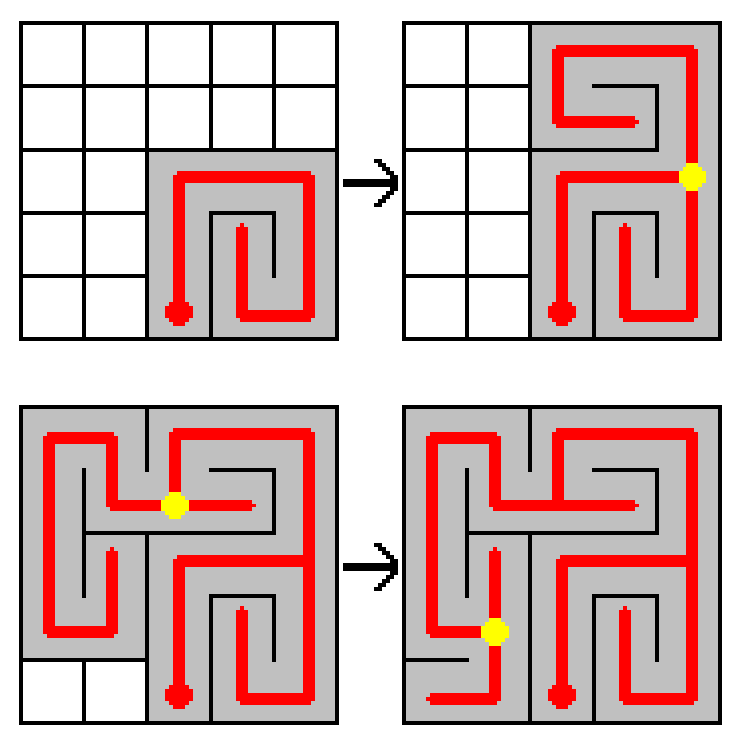
\includegraphics[scale=0.4]{fotos/back_tracker.png}
	\caption{Ejemplo de un algoritmo recursive backtracker \cite{back_tracker}}
	\label{back_tracker_label}
\end{figure}

\subsection{Programación del algoritmo}
\subsubsection{Recursivo}

Desde el punto de vista recursivo, esta forma de contruir un laberinto no presenta grandes problemas. El algoritmo crea una rama del laberinto hasta que le es imposible seguir porque, por ejemplo, el extremo ha quedado ``encerrado'' entre el muro exterior (el cual marca el límite y evita que el programa se salga de la memoria reservada para el laberinto evitando que el S.O. interrumpa la ejecución) y la propia rama. La naturaleza de la recursividad hace que, una vez llegado a ese punto, al no haber posibilidad de movimiento, resuelva por fin esa llamada a la función recursiva y devuelva el resultado a las casillas anteriores que aún estaban pendientes de resolución.  Esto continúa hasta que encuentra una casilla desde la que puede continuar camino, entonces abrirá desde ahí una nueva subrama del laberinto que continuará hasta que quede ``encerrada'' de nuevo y empiece a resolver hacia las casillas anteriores. Puede verse un ejemplo de dicha iteración en la figura \ref{back_tracker_label}. Finalmente, cuando ya no hay más casillas posibles por las que continuar, se volverá hacia atrás todas las casillas hasta llegar a la primera, en nuestro casi siempre la posición $(1,1)$. Este proceso asegura que el laberinto discurra por todas las casillas que sean posibles y que nunca quede encajonado" (como ya hemos dicho, la propia naturaleza de la recursividad lo garantiza).

\subsubsection{Iterativo}

El abordaje iterativo de este problema no es tan sencillo. Esto es debido, al hecho de que crear una rama principal de forma iterativa resulta más complejo que crearla recursivamente. Estableciendo unas condiciones lógicas de control para que la rama no se salga de los bordes y se evite a si misma para no romper el laberinto es suficiente. Pero tarde o temprano, la rama choca consigo misma y no tiene a donde ir. Solucionar este único punto es lo que más esfuerzo supone en la implementación del caso iterativo. La solución más inmedita resulta de crear un nuevo objeto o variable que almacene los lugares por los que la rama (o subrama) ya ha pasado. En esta memoria ha sido la última opción valorada, dado que su implementación significa alejarse del esquema marcado por el algoritmo recursivo. Para ello el equipo se dividió en dos: 
\begin{itemize}
	\item Una persona intentaría resolver el problema mediante la declaración de una variable dinámica local bidimensional. Es decir, una matriz con tantas filas como elementos tuviera la matriz sobre la que se hacía el laberinto y con tantas columnas como las dimensiones del laberinto (2 por ser bidimensional). 
	\item Otra persona intentaría la implementación de una pila dinámica tipo LIFO, que en un principio solo almacenaría los índices de las casillas por las que la rama o subrama había pasado en orden (más tarde se utilizó la pila también para almacenar más datos). 
	\item La tercera persona del equipo ejercería una labor de control y apoyo. Trabajando con las otras dos personas en limpieza del código e implementación de funciones auxiliares. Asimismo, controlaba el desarrollo de las dos vías con el fin de descartar la que menos conveniera para centrar todos los esfuerzos en la más prometedora.
\end{itemize}

Finalmente, la opción elegida ha sido la pila.  

En la primera versión solo almacenaba la situación de las casillas ya ocupadas por la rama. Posteriormente se incluyó una funcionalidad extra en el código: cuando el programa se viera obligado a retroceder por la rama que acababa de construir, comprobaría cada dirección de la casilla en la que estuviera para decidir si era posible continuar en alguna otra dirección, pero de forma que se incuría en algunas ineficiencias, pues se comprobaban direcciones que ya se habían comprobado antes, cuando la rama había pasado por allí por primera vez (o por segunda, o por tercera). Se almacenó entonces en la pila el vector de direcciones aleatorizado, así como por qué iteración iba la comprobación del vector. De esta forma es posible finalizar el laberinto asegurando que todas las direcciones han sido comprobadas y todas en un orden aleatorio.

Se incluye a continuación el diagrama de flujo utilizado para la programación de la función \textsf{Visit()} en el caso iterativo:

\begin{figure}[H]
	\hspace{-4.3cm}
	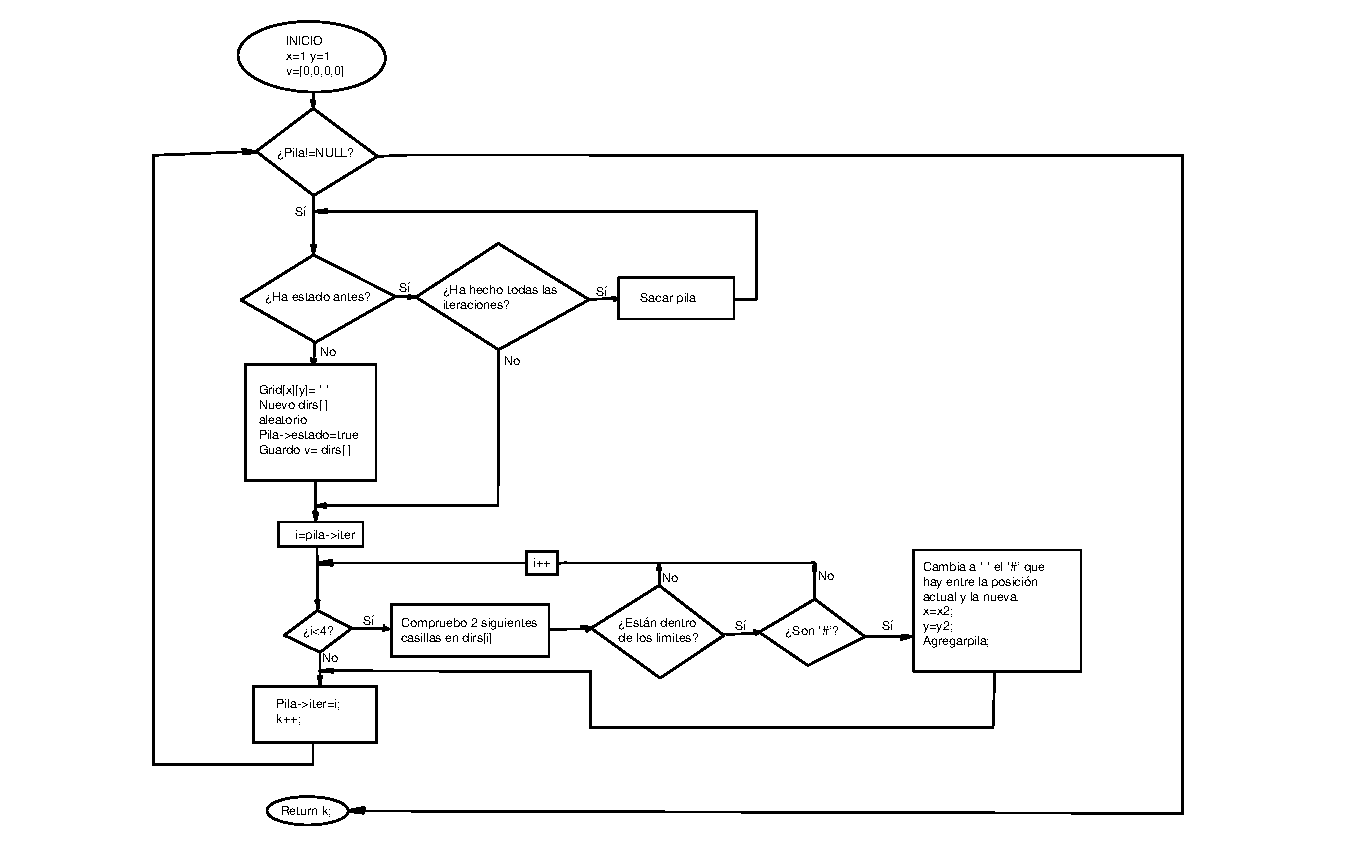
\includegraphics[scale=1.05]{fotos/diagrama.pdf}
	\caption{Diagrama de flujo para la función \textsf{Visit()} en el algoritmo iterativo}
	\label{diagrama}
\end{figure}

\subsubsection{Comentarios al código}

Una vez implementados ambos algoritmos, surgen algunos detalles a ajustar.

Lo primero a corregir fue un ``doble borde'' que aparecía en las paredes derecha e inferior del laberinto. Dichas paredes extras eran debidas a que en la iteración aleatoria por el laberinto la última columna y fila no ``caían dentro'' de los movimientos del programa. Esto a su vez, era debido a que se comenzaba en la casilla $(1,1)$ y que las dimensiones fueran pares o impares. Si por ejemplo, las dimensiones fueran $6x6$, al comenzar en la posición $(1,1)$, y suponiendo que los dos primero movimientos son hacia la derecha, la siguiente casilla a la que moverse sería la $(1,3)$ que sería válida, pero en el siguiente movimiento la nueva casilla estudiada sería la $(1,5)$ que forma parte del borde exterior y no forma parte de los límites o casillas válidas. Por lo tanto, la solución elegida ha sido forzar a que las dimensiones sean siempre impares. Esto no supone demasiado problema, pues el usuario puede pedir dimensiones pares y es el programa quien modifica estas para que sean impares. En concreto las siguientes lineas de código:

\lstset{style=mystyle}
%también se puede poner [firstnumber=39]
\begin{lstlisting}[language=C++, title=Ajuste de dimensiones dentro de la función \textsf{Pedir()}, frame=single, numbers=none]
	// Se ajustan las dimensiones para que sean impares siempre.
    (filas%2) ? filas : filas+=1;
    (columnas%2) ? columnas : columnas+=1;
\end{lstlisting}

de forma que es un cambio transparente para el usuario. Por otro lado, el cambio no es perceptible para dimensiones mayores de $10x10$, lo que es la mayoría de los casos.

Las líneas de código anterior fueron planteadas en su inicio como la \textsc{macro} siguiente: 

\lstset{style=mystyle}
%también se puede poner [firstnumber=39]
\begin{lstlisting}[language=C++, title=Ajuste de dimensiones dentro de la función \textsf{Pedir()}, frame=single, numbers=none]
	#define Arreglar_2D(x,y) (((x%2) ? x : x+=1),((y%2) ? y : y+=1))
\end{lstlisting}
pero finalmente se decidió no utilizar ya que no respondia totalmente a la función de lo que debe ser una \textsc{macro}.

Por motivos estéticos, también se buscó algún carácter en \textsc{unicode} para que las casillas no vaciadas del laberintos se asemejaran más a paredes y poder visualizar el dibujo más fácilmente. Las siguientes líneas de código muestran la posible variante para la función \textsf{PringGrid()}:

\lstset{style=mystyle}
%también se puede poner [firstnumber=39]
\begin{lstlisting}[language=C++, title= Variente para la función \textsf{PrintGrid()} con carácteres \textsc{unicode}, frame=single, numbers=none]
for (int i=0; i<filas; i++) {
    for (int j=0; j<columnas; j++){
    	if(grid[i][j] == '#')
				cout << "\u2B1C";
			else cout << "  ";  // Notese el doble espacio intencionado
		}
    cout << endl;
}
\end{lstlisting}

En las figuras \ref{unicode} y \ref{ascii} puede verse la comparación entre la salida por consola mediante el símbolo \textsc{unicode} utilizado en el código anterior y el símbolo \textsc{ascii} \#.

\begin{figure}[h]
	\centering
	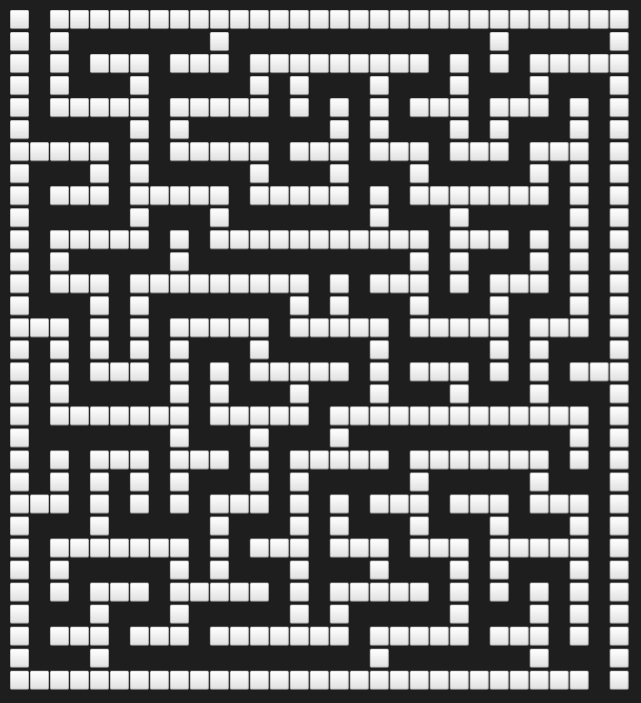
\includegraphics[scale=0.4]{fotos/unicode.png}
	\caption{Salida por consola del programa con carácteres \textsc{unicode}}
	\label{unicode}
\end{figure}

\begin{figure}
	\centering
	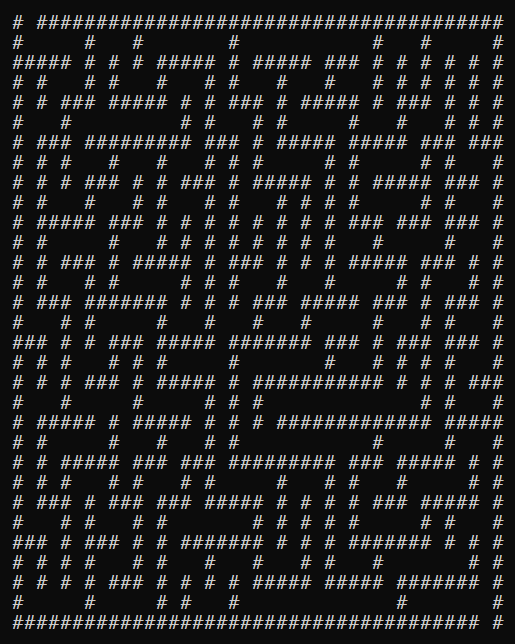
\includegraphics[scale=0.6]{fotos/ascii.png}
	\caption{Salida por consola del programa con carácteres \textsc{ascii}}
	\label{ascii}
\end{figure}

Por motivos de portabilida se ha preferido no incluirlo directamente en el código final. Pero puede ser implementado fácilmente gracias el código anterior.

% \clearpage
\section{Experimentación}
\subsection{Toma de medidas}
Para poder estudiar y comparar la ejecución de ambos códigos y algoritmos, ha sido necesaria una fase de toma de medidas. Los datos buscados corresponden a las diversas métricas empleadas, estas son: número de iteraciones, velocidad de ejecución y uso de memoria. Para la experimentación (esto es, ejecutar el código bajo diferentes condiciones), se ha elaborado un fichero \textit{shell script} que permite ejecutar cada programa repetidas veces y genera un archivo de salida en el que vuelca los datos de cada ejecución. Más tarde este fichero es convertido a una tabla de datos con formato \textit{.csv}. Para su estudio y análisis se ha utilizado la herramienta estadística \textsc{RStudio}.

\vspace{0.2cm}
Más concretamente, el shell script empieza ejecutando el programa con un valor inicial de $20$ tanto para filas y columnas. Y va sumando 50 unidades a filas y columnas con cada ejecución hasta llegar a $10000$, realizando cada ejecución $5$ veces para poder conseguir una media de los tiempos de ejecución. En cada ejecución, escribe en el fichero \textit{output.csv} (o si se prefiere \textit{output.txt}): un número del $1$ al $5$ correspondiente con la ejecución en curso, el tamaño de las filas y columnas, el área del laberinto $(filas*columnas)$, el tiempo empleado en la ejecución de la función \textsf{Visit()} y el número de iteraciones realizadas por dicha función. Se incluye a continuación el bucle principal del \textit{shell script}:
\clearpage
\lstset{style=mystyle}
%también se puede poner [firstnumber=39]
\begin{lstlisting}[language=sh, title= Variente para la función \textsf{PrintGrid()} con carácteres \textsc{unicode}, frame=single, numbers=none]
	initial=20
	final=10000
	step=50
	contador=1
	
	while [ $initial -le $final ]
		do 
			while [ $contador -le 5 ]
			do
				echo -n $contador\ >> $file
				$mypath/Maze_Recursivo $initial $initial 1\ >> $file
				contador=$(($contador+1))
			done
			initial=$(( $initial + $step ))
			contador=$(($contador-5))
		done
\end{lstlisting}
Es importante utilizar \verb|ulimit -s unlimited| dentro del script para evitar que el sistema operativo mate el programa cuando las dimensiones sean demasiado grandes, permitiendo que la pila sea más grande de lo habitual y no llegue a llenarse. Para poder ejecutar el mismo \textit{script} en Windows ha sido necesario utilizar un emulador de Unix (\textit{Cygwin} o una consola tipo \textit{Git Bash}) y cambiar el comando anterior por \verb|/STACK:reserve[10000000]| con la misma inteción.

\vspace{0.2cm}
En la toma de medidas se ha observado que en el recursivo el número de iteraciones es siempre el mismo, ya que al ser constantes las dimensiones del laberinto la función \textsf{Visit()} es llamada el mismo número de veces en cada ejecución con los mismos datos. Pero, por otro lado, las 5 ejecuciones sirven para obtener la media del tiempo. 

\vspace{0.2cm}
En el caso del iterativo, tanto el tiempo como el número de iteraciones varían en cada ejecución. Se cree que esto es debido a la aleatoriedad del recorrido y el vaciado o llenado de la pila. Pues, en el caso recursivo el ``arbol de opciones'' es recorrido de manera sistemática.

\vspace{0.2cm}
A la hora de realizar pruebas, se ha dispuesto de 3 computadoras diferentes: dos  con sistemas operativos vasados en \textsc{unix}, en concreto \textit{Linux}, ambos con diferentes procesadores, y un tercer computador con sistema operativo \textit{Windows 10}. Se ha procedido extrayendo datos de la ejecución de los programas en cada uno de las tres computadores. Lo cual, supone además una manera de comprobar experimentalmente la portabilidad de los programas.

\vspace{0.2cm}
Es importante resaltar en este punto, lo conveniente que ha sido, para la ejecución del \textit{script}, implementar en ambos código el paso de parámetros a la función \textsf{main()}. Se incluye brevemente el código y el paso de parámtros a una función de dichos argumentos:
\lstset{style=mystyle}
%también se puede poner [firstnumber=39]
\begin{lstlisting}[language=C++, title= Implementación de paso de argumentos al \textsf{main()}, frame=single, numbers=none]
	//----FUNCION PRINCIPAL-------------------------------------
	int main(int argc, char **argv){
		// Se pide al usuario el tamano del laberinto.
  		Pedir(argc, argv);
\end{lstlisting}

\section{Análisis}

Gracias a los datos obtenido en la fase de experimentación, se ha podido elaborar una base de datos de tamaño suficiente. La limpieza y el tratamiento de los datos se ha llevado a cabo utilizando \textit{Excel} y el software \textsc{R} en el entorno de desarrollo \textsc{RStudio}. Se ha realizado en varias fases: 
\begin{itemize}
	\item En primer lugar, se importaban los datos a \textsc{RStudio} desde el propio documento de salida, en formato \textit{.csv}, que elaboraba automáticamente el \textit{shell script}. 
	\item Los documentos se inspeccionaban rápidamente mediante gráficos en busca de posibles datos atípicos. Al pasar a través de distintos sistemas operativos era común que las comas decimales se desplazaran, lo que provocaba grandes errores que debían ser detectados.
	\item Solucionado este problema, había que hacer la media de los tiempos, para lo que se ha utilizado la función \textsf{tapply()} de la librería ``tidyvers'', añadir un factor que recogiera el microprocesador utilizado y el sistema operativo en cada ejecución y por último volcar cada tabla de datos a un documento \textit{.csv} de nuevo.
	\item Una vez los datos están tratados y se han volcado en sus respectivas tablas, lo siguiente ha sido unificar en unico archivo dichas tablas. Para poder hacer los gráficos posteriores adecuadamente, ha habido que volver a transformar el dato del microprocesador y el sistema operativo a tipo factor, pues por defecto, \textsc{R} no asigna variables procedentes de una lectura externa a un tipo factor. 
	\item Con la tabla final, se procede a elaborar los gráficos pertinentes. Para ello se hace uso del paquete \textit{ggplot} de la librería ``tidyvers''.
\end{itemize}
 
En el siguiente gráfico (ver \textsc{Fig.}~\ref{grafico1}) se ha representado la evolución del numero de veces que se llama a la función \textsf{Visit()} en función del numero de filas (o columnas) de un laberinto de matriz cuadrada. Como se aprecia, para dimensiones pequeñas (número de filas no mayor que 2500), el algoritmo iterativo y el recursivo presentan un número de iteraciones parecido. Cuando el número de filas empieza a ser elevado, las diferencias entre ambos son notables. A priori, con este gráfico podría decirse que el método recursivo es ``mejor'', pero con solo este gráfico no es posible realizar todavía conclusiones definitivas.

\vspace{0.2cm}
\begin{figure}[h]
	\centering
	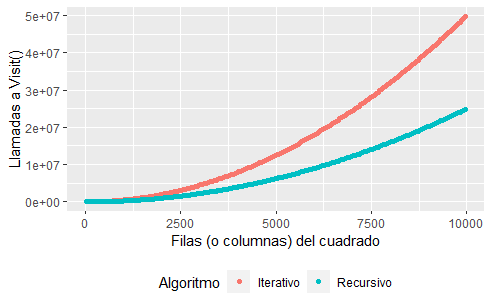
\includegraphics[scale=0.9]{fotos/Iteraciones_vs_filas1.png}
	\caption{Comparativa de número de iteraciones frente a la dimensión de un lado (supuesto el otro igual) para el caso recursivo e iterativo}
	\label{grafico1}
\end{figure}

El siguiente gráfico (ver \textsc{Fig.}~\ref{grafico2}) es en esencia similar al primero. La diferencia más importante radica en que ahora varía el número de elementos del laberinto (el producto $filas*columnas$), no la dimensión de sus filas o columnas. Con este cambio podemos estudiar más adecuadamente el número de llamadas a la función \textsf{Visit()} en el caso de que el laberinto no sea cuadrado. Como puede observarse, la relación entre el número de llamadas y el``área'' de la matriz es lineal y con pendiente aproximada $1/5$ para el algoritmo iterativo y $1/2$ para el recursivo.
\begin{figure}[h]
	\centering
	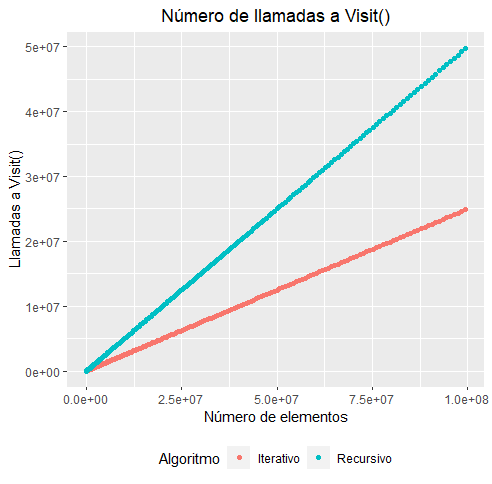
\includegraphics[scale=0.9]{fotos/Iteraciones_vs_numElem.png}
	\caption{Comparativa de número de iteraciones frente a la dimensión de un lado (supuesto el otro igual) para el caso recursivo e iterativo}
	\label{grafico2}
\end{figure}
\vspace{0.2cm}

A la vista de ambos gráficos el algoritmo recursivo resulta más eficiente en cuanto número de iteraciones, tanto con el aumento de filas o columnas, como con el aumento del área ($filas*columnas$). En el gráfico \ref{grafico1} puede aproximarse la evolución de ambos algoritmos por exponenciales, de forma que podemos tener un valor empírico de la complejidad del problema según qué algoritmo.
En la figura \ref{grafico3} puede verse cómo la exponencial ajusta al crecimiento en número de iteraciones (en el caso recursivo) según decrece el orden de la exponencia de $2$ a $1.85$ la cual aproxima muy bien. Podemos concluir que dicho algoritmo es del orden de $\mathcal{O}(e^{n})$ donde $n$ para el caso del recursivo se ha comprobado que corresponde muy parecidamente a $n=1.85=17/20$.

\begin{figure}[h]
	\centering
	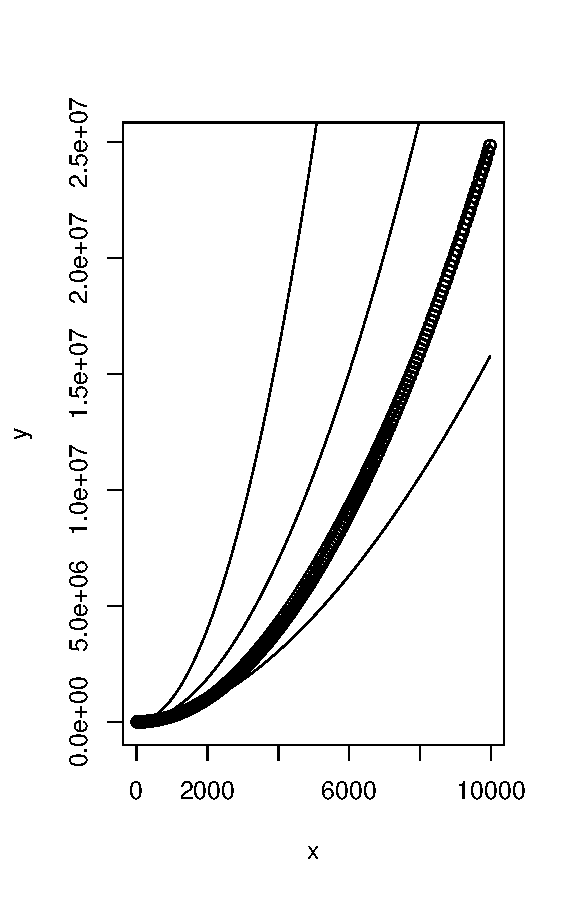
\includegraphics[scale=0.9]{fotos/iterations_rec_vs_pows}
	\caption{Aproximación por exponenciales a la evolución en el algoritmo recursivo del número de iteraciones según el }
	\label{grafico3}
\end{figure}
\vspace{0.2cm}

En los gráficos \ref{grafico4} y \ref{grafico5}, se han comparado los tiempos reales de ejecución completa del programa para los dos algoritmos. Dicha comparación se ha realizado para laberintos cuyo número de elementos es inferior a 100 millones, en tres equipos distintos, de distintas gamas y con distintos años de uso, a fin de mostrar la relevancia de estas características en el desempeño de los programas. Por cuestiones de tiempo no se tienen datos del desempeño del algoritmo iterativo en un equipo con Windows 10 de gama alta (con procesador Intel core I7). Se observa que el algoritmo recursivo es claramente mejor que el iterativo, llegando a recortar en más de dos segundos la ejecución del iterativo en el caso del laberinto más grande evaluado (9971 x 9971 elementos). Lo cual equivale a una mejora sustancial de entre el 31\% y el 33\% respecto al iterativo. Como vemos, el desempeño real es radicalmente opuesto al que pudiera predecirse a partir de los gráficos de las llamadas a la función Visit(). 

\begin{figure}[h]
	\centering
	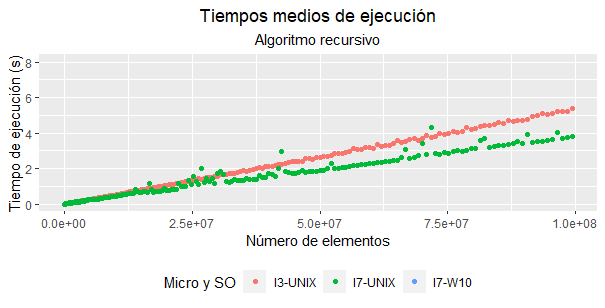
\includegraphics[scale=0.9]{fotos/Tiempos_recursivo.png}
	\caption{Aproximación por exponenciales a la evolución en el algoritmo recursivo del número de iteraciones según el }
	\label{grafico4}
\end{figure}
\vspace{0.2cm}

\begin{figure}[h]
	\centering
	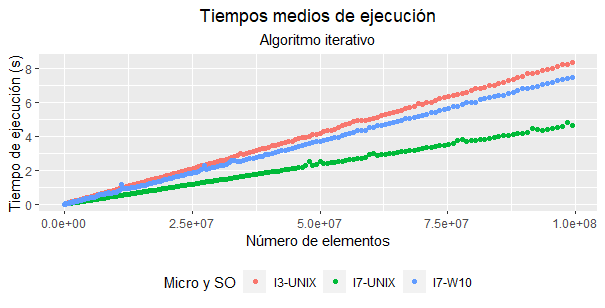
\includegraphics[scale=0.9]{fotos/Tiempos_Iterativo.png}
	\caption{Aproximación por exponenciales a la evolución en el algoritmo recursivo del número de iteraciones según el }
	\label{grafico5}
\end{figure}
\vspace{0.2cm}

Estas notables diferencias son debidas a que los dos primeros gráficos están muy sesgados, pues solo miden la llamada a la función principal de ambos algoritmos, la función Visit(). Si bien esto puede no implicar que su medida incurra en un sesgo importante para determinar cuan bueno es el algoritmo recursivo, sí se incurre en sesgos mayores cuando se trata del algoritmo iterativo. Esto es así porque el mayor peso del recursivo recae en la función Visit(), y la propia naturaleza de la recursividad impone que Visit() se llame una y otra vez a sí misma. Por lo tanto, midiendo la cantidad de veces que se llama a Visit() en el algoritmo recursivo, proporciona una medida útil. Sin embargo, los pesos computacionales del algoritmo iterativo están más repartidos (Visit() llama a otras funciones que no se están contabilizando) y por ende, la medida de la cantidad de veces que se llama a Visit() en este caso, es menos útil, porque es menos extrapolable y comparable, que la misma medida en el recursivo. 

\clearpage
\section{Conclusiones}

\clearpage
\bibliographystyle{abbrv}
\bibliography{mybib}

\end{document}

